\pdfminorversion=7
\documentclass[12pt,authoryear]{elsarticle}

%%%%%%%%%%%%%%%%%%%%%%%%%%%%%%%%%%%%%%%%%%%%%%%%%%
%%%%%%%%%%%%%%%%%%%% PREAMBLE %%%%%%%%%%%%%%%%%%%%
%%%%%%%%%%%%%%%%%%%%%%%%%%%%%%%%%%%%%%%%%%%%%%%%%%

% word count

% references
\usepackage{natbib}

% fonts
\usepackage[default,scale=0.95]{opensans}
\usepackage[T1]{fontenc}
\usepackage{ae}

% colorize links
\usepackage[pdftex,x11names]{xcolor}

% layout control
\usepackage{geometry}
\geometry{verbose,tmargin=1.25in,bmargin=1.25in,lmargin=1.1in,rmargin=1.1in}
\usepackage{fancyhdr}

% math typesetting
\usepackage{array}
\usepackage{amsmath}
\usepackage{amssymb}
\usepackage{amsfonts}
\usepackage{mathtools}
\usepackage{bm}

% float barriers at section ends
\usepackage[section]{placeins}
\usepackage{flafter}

% tables
\usepackage{tabularx}
\usepackage{booktabs}
\usepackage{multirow}

% caption style
\usepackage[font={small},labelfont=bf]{caption}

% footnotes at bottom
\usepackage[bottom]{footmisc}

% enumeration symbols
\usepackage{enumerate}

% graphics
\usepackage{graphicx}
\usepackage[space]{grffile}
\graphicspath{{../results/figures/}}

% sideways figures
\usepackage{rotating}
\usepackage{lscape}

% spacing
\usepackage[doublespacing]{setspace}
\setlength{\emergencystretch}{2em}

% pdf links after footnotes and spacing
\usepackage[pdftex]{hyperref}
\usepackage{xurl}
\hypersetup{hidelinks,hypertexnames=false}

% page template
\setlength{\headheight}{15pt}
\setlength{\headsep}{20pt}
\pagestyle{fancyplain}
\fancyhf{}
\rfoot{\fancyplain{}{\thepage}}

% customizations
\newcommand{\mbs}[1]{\boldsymbol{#1}}
\newcommand{\pkg}[1]{{\fontseries{b}\selectfont #1}}

%%%%%%%%%%%%%%%%%%%%%%%%%%%%%%%%%%%%%%%%%%%%%%%%%%
%%%%%%%%%%%%%%%%%%%% DOCUMENT %%%%%%%%%%%%%%%%%%%%
%%%%%%%%%%%%%%%%%%%%%%%%%%%%%%%%%%%%%%%%%%%%%%%%%%

% remove elsevier preprint note
\makeatletter
\def\ps@pprintTitle{%
 \let\@oddhead\@empty
 \let\@evenhead\@empty
 \def\@oddfoot{}%
 \let\@evenfoot\@oddfoot}
\makeatother

\begin{document}

\thispagestyle{empty}
\begin{frontmatter}

\title{The American Break: Allied Cooperation without the Hegemon}

\author[strath]{Max Gallop}
\ead{max.gallop@strath.ac.uk}
\author[msu]{Shahryar Minhas}
\ead{minhassh@msu.edu}
\address[strath]{Department of Government and Public Policy, University of Strathclyde}
\address[msu]{Department of Political Science, Michigan State University}

\begin{abstract}
\singlespacing
\noindent When Washington turns against policies it once supported, do its allies follow, split, or keep cooperating? Theories of cooperation after hegemony make continuity plausible, while accounts of American isolation establish Washington's departure. We examine what continued through the broad reversal of 2025 by connecting allied cohesion to the content of adopted decisions. Historical General Assembly voting relationships, recurring votes, and requests in successive economic and development decisions distinguish American from allied movement and continued voting support from continued authorization. American vote changes drove the decline in agreement between Washington and its allies. The allies largely kept their votes and agreement with one another, while members renewed most earlier requests despite negotiated revisions. In a body where Washington has no veto, majority rule let members keep authorizing shared work, preserving an avenue for cooperation within the existing order after its leading power changed course.

\vspace{3mm}
\noindent\textbf{Keywords}: international cooperation, hegemony, United Nations General Assembly, UN voting, latent space models, structural change
\end{abstract}
\end{frontmatter}

\newpage\setcounter{page}{1}
\doublespacing
\setlength{\parskip}{0pt}

\section{Introduction}

Canadian Prime Minister Mark Carney called on middle powers to act at Davos in January 2026, describing world politics as undergoing ``a rupture, not a transition'' \citep{carney:2026:davos}. Governments that wanted to pursue policies Washington was abandoning would have to find ways to work together. Their problem also concerns an ambiguity in allied agreement that is difficult to resolve in ordinary times. When allies support the same policies as the hegemon, they could be supporting its leadership or policies they would pursue without it. An American reversal lets us examine the difference. Do the allies implement Washington's new positions, divide over its demands, or continue cooperating on work it now opposes?

The allies had already faced this choice in 2025. After the United States withdrew from the Sevilla preparatory process on development financing, all fourteen allies stayed in the negotiations and later endorsed the resulting commitment in the General Assembly over American opposition \citep{usun:2025:ffd4withdrawal,un:2025:sevillavote}. Governments could still reach a decision together after Washington withdrew its support. The political significance of such decisions depends on what happened beyond the individual dispute: whether the partners stayed together and whether the work they authorized survived negotiation.

Theories of international order give us good reasons to expect some cooperation to continue. In the debate over the establishment and maintenance of order \citep{gilpin:1981}, \citet{keohane:1984} and \citet{snidal:1985} explain how cooperation can survive a decline in the hegemon's power. \citet{ikenberry:2001,ikenberry:2011} places the rules and relationships through which governments pursue shared policies at the center of that order. A reversal of American policy brings an additional problem into view. The institution and its procedures are still available, but members seeking to renew a negotiating mandate or request for resources must now decide whether to pursue work Washington opposes. Renewing those requests is a political choice within the inherited order.

\citet{voeten:2026:usdeparture} documents Washington's departure in 2025 and provides the nearest empirical starting point.\footnote{The Assembly's record has supplied evidence of resistance to American dominance \citep{voeten2004resisting} and accommodation of American interests \citep{kegley:hook:1991,carter:stone:2015}. Related work examines changing alignment during the first Trump administration \citep{mosler:potrafke:2020} and a recent American turn away from its alliances \citep{carson:metz:poast:2025}.} Earlier episodes of allied defiance make the breadth of the American reversal the distinctive feature of 2025. Yet an isolated Washington could leave behind partners who disagree with one another, or a majority that stays together by giving up earlier work. Establishing American isolation therefore leaves a consequential question about the cooperation among the other governments. Our contribution is to connect their voting relationships to the actions their decisions continued to authorize.

A decline in bilateral agreement can originate with either government, so we develop a dynamic network model that estimates countries' relationships jointly from 1989 through 2025, allowing each country to break from its earlier path in a different year. Recurring votes then identify which government changed its vote on questions recorded in both years. However, a recurring title keeps a question in view without holding its policy content fixed. Following the actions requested of governments and UN bodies through successive economic and development decisions establishes whether members preserved the earlier work. 

We find considerable continuity among Washington's partners and in the adopted work. The model fitted to the full weighted agenda favors an American break in 2025 and continuation for all fourteen allies, a classification that depends on the recorded agenda and vote weights. More directly, the allies kept 191 of their 194 earlier votes on recurring resolutions where Washington switched, and their agreement with one another barely changed. Most earlier requests in the economic and development decisions continued unchanged, despite negotiated revisions and concessions. Authorization by the Assembly's membership is separate from cohesion among the fourteen allies. Tax cooperation makes the distinction clear: the adopted decision retained the negotiating mandate while all fourteen allies abstained. The governments authorizing continuing work can vary across decisions.

Majority rule gave members a means of pursuing policies within the existing order after its leading power changed course, in a body where Washington has no veto. The first year's response is compatible with patient bargaining, in which allies wait for American policies to change again, as well as with more durable support for the policies themselves. Establishing the origins and duration of that support, or the institution's causal role in sustaining it, requires further evidence. Financing and implementation require decisions beyond adoption. The more difficult political choices concern work that requires resources Washington supplies or action it can block.

We first consider the possible foundations of allied agreement. The voting analysis then locates the American departure and examines the allies' response, before the adopted decisions establish what work survived negotiation. The discussion returns to the choices facing governments that seek cooperation after the hegemon changes course.

\section{What allied agreement rests on}
\label{sec:theory}

An ally can vote with Washington in exchange for security or economic benefits, because it expects their bargain to endure a temporary quarrel, or because it supports the policy itself. These explanations lead to the same observed agreement while American and allied policies coincide. After an American reversal, what counts as evidence for a voting bargain will depend on when the allies have reason to respond and on the costs they face for defiance.

Vote buying research has detailed when and how such incentives and penalties are offered up in Assembly votes \citep{carter:stone:2015}. A voting bargain gives an ally reason to adopt new American positions when Washington offers inducements or threatens penalties. If support depends on the bargain and defiance is costly, allies should change their votes when Washington seeks support; different responses could also divide them. Indeed, in 2025, Washington in its explanation of position \citep{usun:2025:longform} laid out the revisions it sought in Second Committee texts. We can thus monitor the behavior of the ally in question in the very same set of resolutions in which Washington demanded such support. The statement identifies desired revisions without establishing a threat attached to every Assembly vote.

Authority can also permit resistance. \citet{lake:2009} treats it as an exchange in which the hegemon provides order and exercises restraint; \citet{lake:2018} explains how divergent interests and lost legitimacy can undermine it. Other powers can maintain the earlier bargain's positions while expecting American policy to change again. They may resist an arbitrary reversal without abandoning the relationship. Their first-year votes could therefore resemble those of allies supporting the policies independently of the bargain.

As for support of policies for reasons unrelated to the original sponsor, institutions can grant their members opportunities to negotiate and authorize programs which they themselves wish to pursue \citep{keohane:1984,ikenberry:2001}. They would continue to support such policies on recurring issues by casting unchanged votes and agreeing with one another. Allies would also back work with other members when Washington votes no on a newly recorded question. The Assembly's familiar negotiating procedures and majority rule would let members renew earlier requests in subsequent decisions. We follow the adopted decisions to see what continued. Showing that the institution caused that continuity would require evidence of how it changed governments' choices.

An ally's reasons for supporting a policy may also have developed within its relationship with the hegemon. \citet{ikenberry:kupchan:1990} explain how governments can adopt norms promoted by a hegemon, giving those norms a possible role in support after its reversal. Of course, socialization, preference convergence and patient bargaining could all produce unchanged votes in the first year. The votes let us distinguish continuity from immediate following and division, while further evidence is needed to account for where support came from and how long it will last.

In the December 2017 Jerusalem debate, Nikki Haley warned that Washington could redirect contributions in response to the Assembly's treatment of American positions \citep{un:2017:jerusalem}. Eleven allies nevertheless voted yes against an American no; Australia, Canada and Poland abstained. Defiance there can be inexpensive: Washington has no veto, and allies can disagree while cooperating in security and trade. These conditions bound our first-year test in 2025.

The EU provides another reason to examine continuity beyond the group as a whole. Eight of our fourteen allies are members, and they coordinate their Assembly votes. \citet{burmester:jankowski:2014} examine both that coordination and the disagreements that persist. We therefore follow the six non-EU allies separately to see whether continuity extends to them too. Stable votes outside the EU would extend the result beyond its members, although this would still leave coordination's contribution unidentified.

Table~\ref{tab:typology} sets out the possible responses. We also compare American alignment with nine rivals: Belarus, China, Cuba, Iran, Nicaragua, North Korea, Russia, Syria and Venezuela. Countries can move together below the individual break threshold, so we assess allied following and division through their votes and within-group agreement alongside break probabilities.

\begin{table}[ht]
\centering\small
\caption{Possible responses to an American reversal and the 2025 evidence}
\label{tab:typology}
\begin{tabularx}{\textwidth}{>{\raggedright\arraybackslash}p{.19\textwidth}>{\raggedright\arraybackslash}p{.34\textwidth}>{\raggedright\arraybackslash}X}
\toprule
Response & Observable implication & Evidence for 2025 \\
\midrule
Allies follow Washington & Votes change toward the new American vote & Allies kept 191 of 194 votes on recurring questions where Washington changed \\
\addlinespace
Allies divide & Agreement among the allies falls & Agreement of 93.2 percent in 2024 and 93.4 percent in 2025 on recurring questions \\
\addlinespace
The United States joins its rivals & American agreement with the rivals rises & Full-agenda agreement fell; the February Ukraine votes are an exception \\
\addlinespace
A wider realignment occurs & Many countries break independently from their earlier positions & Expected non-US breaks among regular voters of 0.3 in the released weighted fit; classifications depend on weights \\
\addlinespace
Cooperation continues without American support & Allied votes persist and adopted decisions keep earlier work & Unchanged requests of 81.3 percent, averaged over 24 initiatives \\
\bottomrule
\end{tabularx}
\end{table}
\FloatBarrier

Finally, a resolution with the same title and majority could still lose its negotiating mandate or request for resources. We track requests for meetings, reports, etc. in subsequent decisions on the same text, including any revisions that may be negotiated in the text itself. Financing and implementation come later in the cooperation process.

\section{Measuring who moved}
\label{sec:model}

\subsection{The voting record}
\label{sec:votes}

The voting record includes all recorded General Assembly votes for 1989 through 2025. We draw this from the UN Digital Library database, using its version of 6 February 2026. For every country-pair, we then computed agreement by scoring identical votes as 1, an abstention paired with either yes or no as 0.5, and opposite yes and no votes as 0. Nonvotes by either country are missing. For descriptive purposes, we first averaged the above scores for all resolutions on which a country-pair did vote, and then gave every country-pair equal weight. However, for the network model, we gave more weight to those votes where the General Assembly was more evenly divided. We computed these weights from the Yes and No totals for each vote. In a robustness check, we therefore recomputed these weights without the American vote. \footnote{The supplement gives the weighting formula and repeats descriptive comparisons using only identical votes or only yes and no votes. These are agreement rates; \citet{hage:2011} discusses adjustment for agreement expected by chance.}

We set the rule for this fixed comparison group after examining the 2025 votes. Membership requires a mutual defense treaty with the United States continuously in force from 1 January 2001 through 2025, high-income status in the World Bank's July 2026 classification, and 2024 GDP of at least 400 billion dollars in the October 2026 World Economic Outlook. \footnote{The supplement records each criterion and sensitivity. Poland joined NATO in 1999; earlier comparisons follow the same fourteen states.} The supplement reports selection sensitivities, exclusions and country coverage. The model includes every Assembly member; break counts use regular voters, those casting at least three-quarters of a year's recorded votes.

The voting questions put to a recorded General Assembly vote changed sharply in 2025. To examine whether a shift in a country's national positions has occurred from year to year we will compare the country's voting in a given year to its voting in another year, for a set of recurring resolutions that have the same title in both years. The annual nuclear-test-ban treaty resolution, for example, holds a recurring question in view instead of comparing unrelated items. Applying the same rule throughout the record lets us judge the American change in 2025 against earlier years. \footnote{The comparison requires unique recurring titles and recorded votes by both countries in both years. The supplement gives title matching, country-specific denominators, resolution-weight ranges and the replacement accounting.} This also means that a resolution with a repeated title can contain very different decisions from year to year. We therefore read every recurring resolution on which the United States changed its vote in the comparisons ending in 2025, together with all 33 resolutions adopted without a vote in 2024 and decided by recorded vote in 2025.

A request is defined as an action assigned to an identified government or institution to undertake a task such as to prepare a report, call a meeting or to implement a mandate. In order to monitor the content of decisions in the Second Committee over time, all such requests are followed through successive decisions, including the relevant resources and timescales. Continued and changed content are reported in Section~\ref{sec:proposals}.

\subsection{A model of country-specific breaks}

How do we look for a break in all of a government's relationships? Looking for a fall in agreement within a pair of countries is not sufficient since such a fall could be caused by a break by either country. The recurring votes tell us which government changed on those questions; we examine them directly in Section~\ref{sec:votes-behind}. We also develop a model that helps us to address the attribution problem for all governments.

Consider Germany, with about 190 voting relationships in a given year: a sharp decline in agreement with the US, while agreement with the rest of the world stays stable, would give us little reason to classify Germany as breaking from its earlier path. On the other hand, a sharp decline in US agreement with almost all countries would make an American break more plausible. Thus, we employ the relationships of each country with the rest of the Assembly, over time, to distinguish between a country's own break and the change in a partner's position.

Our extension can be viewed as a combination of two approaches for describing change at different levels. First, ideal-point-based estimation as well as smooth dynamic network models can model countries on a smooth path that changes over time \citep{bailey:strezhnev:voeten:2017,sewell:chen:2015}. In contrast, network changepoint models can model the entire network as changing all at once \citep{park:sohn:2020}. We estimate a model in which each country either drifts or breaks in a year, with all countries' relationships estimated jointly. Thus, countries can break in different years.

Each country has a position in two dimensions in each year, much as an ideal point summarizes a legislator's voting record. We use that position to summarize agreement with other countries after accounting for the country's average tendency to agree over the whole period \citep{hoff:2021,minhas:etal:2019}. We hold that average fixed across years, so changes in expected agreement over time enter through the positions. For countries $i$ and $j$ observed in year $t$, weighted annual agreement follows
\[
y_{ij,t}\sim\mathcal N\!\left(\mu+a_i+a_j+u_{i,t}^{\mathsf T}u_{j,t},\ s^2\right),
\]
We can read the fitted agreement in two parts. The common level $\mu$ and country effects $a_i$ and $a_j$ supply a baseline for the pair; the inner product of $u_{i,t}$ and $u_{j,t}$ captures what those terms leave unexplained. Positions pointing in the same direction from the origin imply higher agreement than that baseline predicts. The plot displays the positions, so it leaves out the common level and country effects that also enter the fit. Distance in the plotted space therefore gives only a partial account of alignment.

We then allow two ways for a position to change. Under drift, it continues from the previous year with a random step; under a break, it is drawn independently of its earlier position:
\[
u_{i,t}\mid\delta_{i,t},u_{i,t-1}\sim
\begin{cases}
\mathcal N(\rho u_{i,t-1},\sigma^2 I), & \delta_{i,t}=0 \quad\text{(drift)},\\
\mathcal N(0,\kappa^2 I), & \delta_{i,t}=1 \quad\text{(break)},
\end{cases}
\qquad \delta_{i,t}\mid\pi\sim\operatorname{Bernoulli}(\pi).
\]
For drift, we estimate persistence $\rho$ and step size $\sigma$ from the data. For a break, we draw the position afresh with $\kappa=2$. \footnote{The supplement and the replication files call a break a ``reset''.} A $\operatorname{Beta}(1,999)$ prior on the break rate $\pi$ has a mean of one break per thousand country-years, making breaks rare unless the voting relationships support them. Without a break the model becomes a smooth dynamic network model. The extension gives us $\Pr(\delta_{i,t}=1\mid\text{data})$, the posterior probability of a break for each country and each year after the first. Values near one favor an abrupt departure from the earlier path, while values near zero favor continuation. \footnote{The estimated break concerns a country's voting relationships. Its political interpretation requires examination of the underlying votes, including changes in the questions being decided.}

At the posterior means, a rho-adjusted move of about 0.23 units favors a break. The American move was 0.29 in 2025. The estimated step size of the drift is 0.049, the persistence is 0.98998 and the break rate is 0.028. The fresh positions are drawn at the break scale of 2, i.e. they spread out over a wider area than the positions actually observed in the data. We derive the threshold for classification and examine the break scale in more detail in the supplement. Persistence lies at its prior's bound of 0.99, a constraint to keep in mind when interpreting the estimated drift distribution.

As noted above, the estimation of a time-constant common level and country effects also matters for the interpretation of the results. With the common level and country effects fixed over time, a country's position must absorb changes in its overall agreement. A high break probability alone therefore cannot separate a level change from a directional one. For the US in 2025, a common fall in agreement accounts for 78 percent of the squared fitted change across partners. On the other hand, a low probability of a country's break does not rule out the possibility that such a country has changed its positions in a way that is confined to a subset of its partners. Thus, in addition to the results from the estimation of the main equations, we also examine recurring votes and agreement within the allied group to assess following and division directly.

The votes included in the network also affect results. A fit of the last two years on the 59 titles that were recurring yielded an American break probability of 0.00012. Giving resolutions equal weight puts all fourteen allies above one half along with the United States. The recurring-title fit locates the full-agenda classification in the expanded set of recorded disagreements. The equal-weight fit shows why the classification depends on the questions receiving weight. We interpret the full-agenda model with recurring votes and agreement within the allied group, which give the direct evidence of continuity. The supplement gives informative checks, and replication materials retain the complete analysis record.

\subsection{What the estimates can establish}

We highlight three areas of concern in performing these checks: (1) new issues going to vote, (2) data uncertainty associated with countries voting infrequently, and (3) a partner's change being attributed to the wrong country.

First, simulated networks let us decide which countries break and when, then ask whether the model finds those breaks and avoids others. We find that it separates drift from breaks as large as its break component assumes when many countries break at once. This includes breaks in the final period, where 2025 sits in the observed record. Smaller single-country breaks are harder to detect. With a probability above one half defining detection, the model finds 57 of 60 fitted-size breaks planted in a quarter or half of the countries at once, against 2 of 6 single-country breaks at a quarter of that size. Changing the questions put to a vote can also produce apparent breaks even if each country's vote on every question stays fixed. Following recurring resolutions lets us check the American change on questions observed in both years. \footnote{The simulated break scale is 2, against an American move of 0.29. The supplement reports detection by size, number of countries and timing; terminal estimates have no later observations with which to assess persistence.}

To limit the effects of countries with few votes in a year we only count breaks for countries that vote regularly. A country with few votes has an uncertain position and can receive a high break probability for that reason alone. \footnote{Country-year comparisons require observed relationships in both adjacent years. The supplement reports participation distributions, alternative cutoffs and sensitivity to the common break rate.}

We then ran the same model on the data for the year 2024, holding the 2024 network fixed except for American relationships, which were replaced by their full-agenda 2025 values. The result for the US was a break probability of 0.9997, while favoring continuation elsewhere. Thus even when a change in a country's relationships with its allies was confined to its relationships with the US, our model attributed that change to the US alone. \footnote{The released full-network fit uses four chains and passes the convergence checks: maximum $\widehat R=1.0022$, minimum bulk effective sample size 924 and minimum tail effective sample size 1,677. The supplement reports all fits, priors and simulations.}

\section{The American break and allied continuity}
\label{sec:break}

We start with the estimated voting relationships and then examine the recurring questions behind them. The two kinds of evidence let us identify the American departure and follow the response among its partners.

\subsection{The United States broke alone}

In the released weighted fit, the 2025 American break has probability 0.998; no earlier American transition has a probability above 0.001. The highest among the allies is 0.020, for the United Kingdom. \footnote{The joint posterior probability that 2025 is the first American break is 0.996, averaging the conditional event probability across draws.} Thus, under the agenda and weights used here, the fit clearly separates an American break from allied continuation. This is compatible with considerable allied movement: nine of the fourteen made their largest estimated move in their own records in 2025. Across all fourteen, the rho-adjusted displacements of 0.118 to 0.185 units were 41 to 64 percent of the American move. Every one was below the common displacement threshold, which explains their low break probabilities despite the size of their moves by their own historical standards. Among other regular voters the full-agenda fit expects 0.3 breaks, fewer than in 26 of the 35 earlier years.

This common classification also makes the historical comparison possible. The model favors drift for the United States at every earlier transition, including 2017 to 2020, and identifies joint breaks among related countries in other years. Ending the fit in 2020 still favors American continuation. Similarly, restricting the likelihood to regular voters favors an American break in 2025 and continuation for all fourteen allies. Simpler full-agenda measures and dynamic ideal points also rank the American change in 2025 highest in its own history. We can therefore locate the departure in both the network and the American record, while retaining the sensitivity to agenda and weights explained in Section~\ref{sec:model}.

\subsection{The allies stayed together; the United States did not join its rivals}

Figure~\ref{fig:space} shows estimated positions in 2024 and 2025 for the United States, its allies and its rivals. Near the allies in 2024, Washington stands apart from both allies and rivals in 2025, while the allies remain clustered together. American agreement with the 14 allies on the full agenda decreased from 70.9\% in 2024 to 23.8\% in 2025, and agreement with the nine rivals decreased from 24.9\% in 2024 to 11.2\% in 2025. In both cases, the level of agreement was below the lower bound of their respective 1989--2024 ranges. Washington's movement away from the allies was not a movement toward the rivals as a group. \footnote{These levels follow each full annual agenda, holding neither the questions nor the observed countries fixed. The supplement reports their earlier averages and ranges.}

\begin{figure}[!ht]
\centering
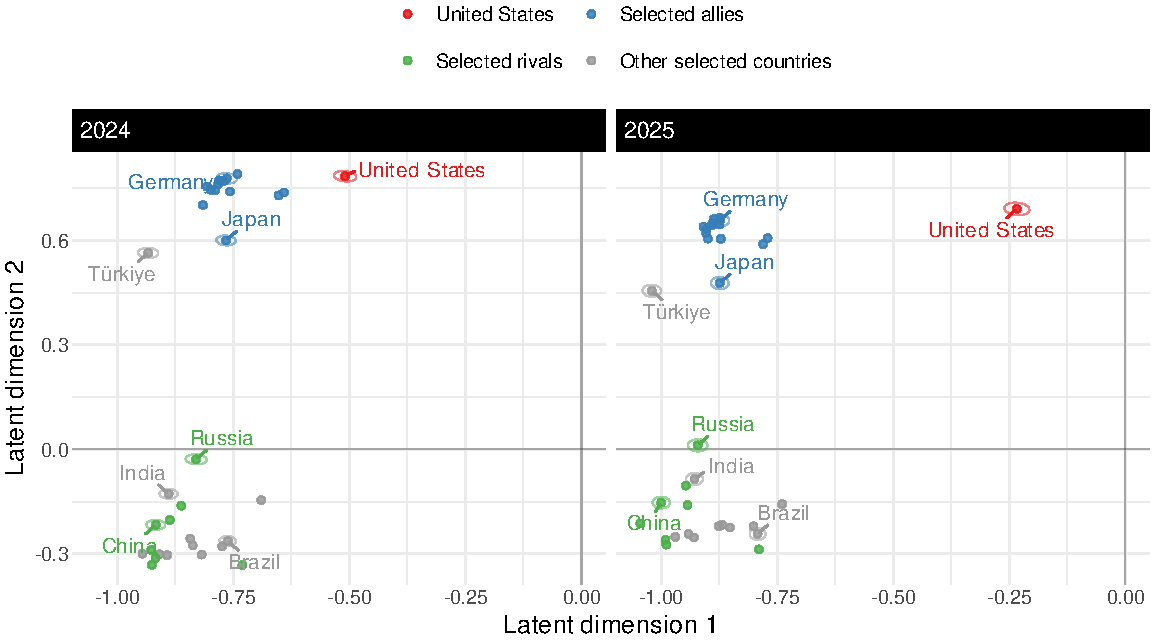
\includegraphics[width=\textwidth]{cooperation_space.pdf}
\caption{Estimated UN voting positions in 2024 and 2025. Points show posterior mean positions from the dynamic UN voting model. The United States is red; the selected groups of fourteen allies, nine rivals (including Russia, China and Iran) and eleven other large countries (including India, Brazil and T\"urkiye) are blue, green and grey. Only the 35 selected countries are shown; Venezuela has no 2025 ties. Ellipses summarize 95 percent of the aligned draws for labeled countries. Each year is rotated or reflected to the same reference frame; distances and fitted relationships are preserved. The horizontal axis is expanded for readability. Fitted agreement depends on more than distance alone.}
\label{fig:space}
\end{figure}
\FloatBarrier

Comparing the European allies with the Indo-Pacific allies on recurring resolutions, agreement changed by less than a tenth of a percentage point between 2023 and 2025. In contrast, agreement by the US with the European and Indo-Pacific allies of the US declined by 17 percentage points between 2023 and 2025. \footnote{The supplement reports each country and regional group separately, including the increase in Canadian agreement and the declines for some European allies.}

For another measure of their movement, we look at the Assembly as a whole. In 2025 the fourteen allies moved together toward the rest of the membership (Figure~\ref{fig:space}). Moving together can preserve internal agreement while changing relations with other members, without a break. Following Washington on particular questions would also appear as drift, so Section~\ref{sec:break} examines the votes directly. On the full recorded agenda, the gap between agreement within the allied group and agreement with members other than the United States fell from about 25 percentage points in 2024 to about 13 in 2025, the largest annual decline. On recurring resolutions, however, it was about twenty-seven points, with little change from 2023 or 2024. \footnote{The gap between the allies' agreement with one another and their agreement with other non-US countries also persists when recurring resolutions receive equal weight.} Items without a recorded vote under the same title in 2024 account for the difference. Washington almost always voted no while the allies generally joined other members. Of the 33 resolutions that were put to a vote in 2025 that had not had a same-titled resolution put to a vote in 2024, the United States voted against 32 of them; the allies as a group voted in favor of 438 of 462 such votes. On these resolutions the agreement of the allies with other members was 96.2 percent, a number about the same as their 96.0 percent agreement with each other on these same newly recorded resolutions. Most of the fall in the gap comes from another 101 items lacking a same-title match to a 2024 resolution. Washington voted no on 95, and the gap on these items was about 8 points. \footnote{The supplement reconciles the 192 archive items with 187 regular-session resolutions, four emergency-session resolutions and one decision. The adoption-list match leaves 58 recurring recorded titles because one title has both a recorded and an unrecorded adoption in 2025.} The questions reaching a recorded vote thus shape the joint move. The allies kept their votes on recurring questions and usually supported the texts Washington opposed on newly recorded questions.

High cohesion over Assembly resolutions coexisted with disagreements over individual texts. The European Union accepted consensus on the Conference on Disarmament's report in 2023 while objecting to deadlock and excluded observers \citep[p.~35]{un:2023:p3record}. In 2025, a Dutch-led group including Belgium, Canada and Denmark withheld support on similar grounds, thereby dividing the fourteen Allies while the US voted yes \citep{netherlands:2025:cd}. This disagreement over a text coexisted with allied continuity when Washington reversed its votes.

The 24 February 2025 Ukraine resolutions were an exception to declining American agreement with the rivals. All fourteen allies voted yes on A/RES/ES-11/7 and A/RES/ES-11/8; the United States voted no alongside Russia on the former and abstained on the latter. Across the full agenda, many development and human-rights texts drew support from the rivals and opposition from Washington. The decline in aggregate agreement thus coexisted with American cooperation with Russia on these Ukraine votes.

\subsection{The American break in historical perspective}

The model further allows us to include in the comparisons of voting behavior over time other historical transitions, including the end of the Cold War, 2000--2002, and the first Trump term. Note that Poland's transition from the lower group containing the Soviet Union to the allied group occurred between 1989 and 1992. The American position on the full agenda changed very little over the four years of the first Trump term, and, indeed, the longest arrow in the final panel is for the US in 2025, although that panel spans only one year. The allies move down and to the left together and end near one another.

\begin{figure}[p]
\centering
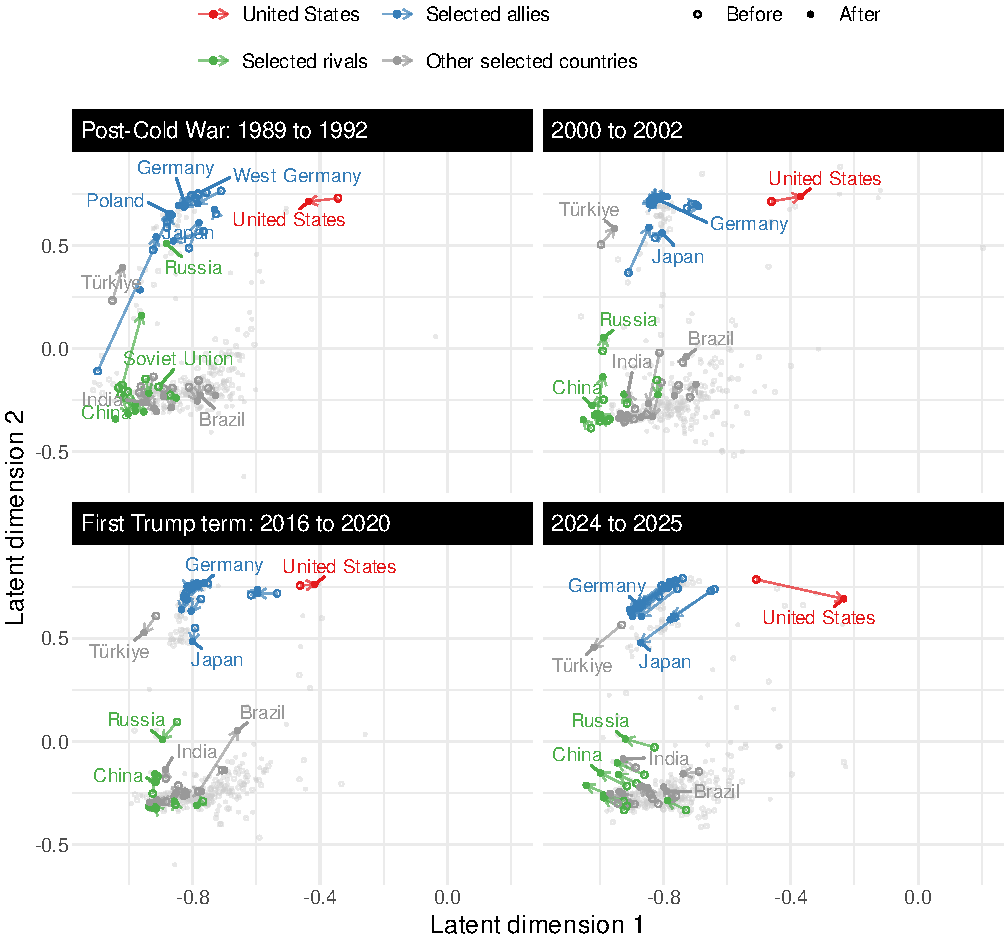
\includegraphics[width=\textwidth]{historical_space_shifts.pdf}
\caption{Changes in estimated UN voting positions across four historical intervals. Open circles mark the starting year, filled circles the ending year, and arrows connect countries observed at both endpoints. Selected countries retain the colors of Figure~\ref{fig:space}; other countries appear in pale grey. Each year is aligned to the same 2024 reference. The intervals differ in length, so arrow lengths describe change over each named interval rather than comparable annual rates. Countries that entered or left the voting record during an interval appear only at the endpoint where they are observed. GER denotes West Germany, which the model keeps separate from DEU. The horizontal axis is expanded for readability. Arrows join posterior means rather than representing separate tests of change.}
\label{fig:historical-space}
\end{figure}
\FloatBarrier

For the Cold War end the model classifies as joint breaks the five East European countries in 1990 (Bulgaria, Czechoslovakia, Hungary, Poland and Romania), and the Soviet Union, as well as the two Soviet republics with their own UN seats (Belarus and Ukraine) in 1991. In 2000 the model classifies as a joint break Russia, together with Belarus and Kazakhstan. The fourteen allies have no such joint break in 2025. \footnote{The supplement and replication tables retain all historical country-year classifications, including Serbia and Argentina.}

The model can classify related countries as breaking in nearby years without telling us why they were aligned. Regime change coincided with the five East European breaks in 1990; the Soviet break followed in 1991. Argentina moved toward Washington in its breaks of 1991 and 2024, before the American reversal in 2025. Comparing Washington with its own record is more direct: the 2025 change exceeds the earlier ones, whereas allied continuity on recurring questions also characterized the first Trump term.

\subsection{Washington changed its votes while the allies kept theirs}
\label{sec:votes-behind}

These same recurring resolutions show a marked contrast between the US and its fourteen allies. Agreement between the US and its fourteen treaty allies fell from 68.0\% in 2024 to 51.1\% in 2025 while agreement among the fourteen treaty allies remained roughly constant at 93.2\% in 2024 and 93.4\% in 2025.

The fall in American agreement with the fourteen allies in the upper panels of Figure~\ref{fig:matched-history} lies below every earlier change, while agreement among the allies in the lower panels changes little in any year. The change under our main measure is a decline of approximately 17 percentage points, against some 4 percentage points for the largest previous decline, and even measuring from 2023 the change would be a decline of approximately 17 percentage points or the largest two-year fall. Excluding abstentions gives a fall of approximately 13.3 percentage points or even larger than the largest previous fall of 3.6 percentage points in 2001. The decline was thus more than a reversal of unusually high agreement in 2024. \footnote{Reweighting recurring resolutions gives annual declines of about 10 to 26 points under the primary score. Alternative rules retain declines, although the historical ranking varies under some reweightings.}

\begin{figure}[ht]
\centering
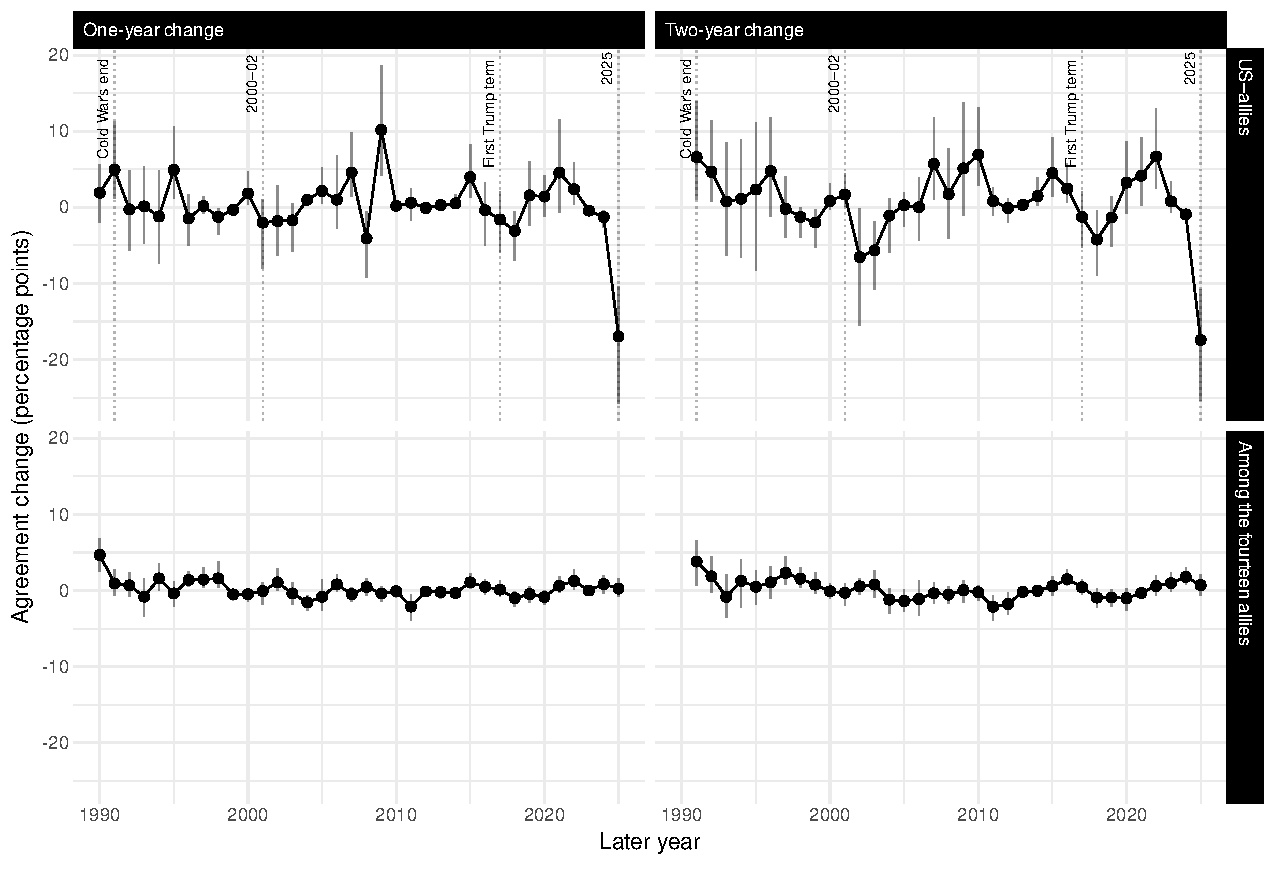
\includegraphics[width=\textwidth]{allied_history.pdf}
\caption{Change in agreement on recurring resolutions, for US--ally pairs and for pairs of allies. The US--ally decline in 2025 lies far below every earlier change, while agreement among the allies changes much less. Each comparison follows the same recurring resolutions for each country pair across its two years. The ranges show how the estimates vary when the recurring resolutions are reweighted. Dotted lines mark historical reference points, not model-estimated break dates.}
\label{fig:matched-history}
\end{figure}
\FloatBarrier

Replacing earlier votes one country at a time assigns 15.79 of the 16.95 percentage points of lost agreement to American changes. The allies kept 191 of their 194 votes from 2024 on recurring resolutions where Washington switched. \footnote{The supplement reports the decomposition and earlier American reversals.} They had also usually held their votes through earlier American reversals, including those of the first Trump administration. What stands out in 2025 is how far Washington reversed course.

Following the same resolution title does not hold its decisions constant. Most texts on which Washington reversed contained substantive updates or different decisions. For example, the Palestine-refugee resolution renewed UNRWA's mandate through June 2029, a decision absent from the 2023 and 2024 texts. The nuclear-test-ban resolution offers the other kind of case: its core requests persisted while Washington changed its vote. The seventeen-point decline consequently covers disagreement on continuing commitments as well as revised decisions within recurring resolutions. \footnote{Three of the fourteen switched titles retained their central requests and account for 3.40 of the 16.95 points lost, with all 42 allied votes unchanged. The supplement reports the text comparisons and the longer-baseline result; this narrower subset has no comparable historical text coding.}

Newly recorded votes for previously unrecorded adoption of texts by the General Assembly also provide evidence of disputes not recorded before. \footnote{Root mean squared change among non-US countries ranks first across the full recorded agenda and fifteenth among 36 transitions on recurring questions. The supplement gives the construction and comparisons.} There were 33 new recorded votes on the 33 newly recorded resolutions that all were adopted by the General Assembly. The allies voted yes on 438 of 462 votes, while the United States voted no on 32 of the 33 resolutions. \footnote{The supplement reconciles the adoption lists and voting archive. A requester is established for 2 of the 33 new recorded votes; other delegations also requested votes, including on A/RES/80/65.} Members adopted these resolutions over Washington's opposition, showing cooperation without American support. The next section follows their texts. What are governments and UN bodies being asked to do on these issues covered by the resolutions?

\subsection{Few other members followed Washington}

Of the members outside the fourteen, few agreed with the change in the US position on recurring resolutions. In total 2,307 paired votes were recorded for members outside the fourteen. Of these 2,241 or 97.1\% remained unchanged. In 45 cases or 2.0\% of cases where there was room to agree with a change in the US position on a recurring resolution, members outside the fourteen agreed with the change while in 21 cases they moved away from the new American vote. Only eight members followed on two or more recurring resolutions: Argentina (6), Israel and Paraguay (5 each), Fiji (4), and Burundi, Hungary, the Marshall Islands and Papua New Guinea (2 each). Movement was concentrated among particular governments and questions, including Palestine-refugee assistance and the International Criminal Court's report.

We find no evidence that treaty allies followed Washington more frequently. NATO members on average moved toward the US in only 2.1\% of the instances in which they could have done so. Similarly, the five Pacific treaty allies moved toward the US in none of 70 eligible cases. On average, the EU members moved toward the US in 1.9\% of all instances in which they could have moved toward it. All other members on average moved in 2.0\% of the instances. Six of the non-EU allies of the US collectively retained all of their 84 paired votes, while the eight EU members collectively retained 107 out of 110 paired votes. Hence, even beyond the EU there is considerable continuity. As mentioned before, this is compatible with patient bargaining, and with support for the content of these policies.

On the 33 newly recorded resolutions, Israel and Argentina each voted NO on 11 of the Washington opposed resolutions, with Paraguay voting NO on 4 of them. These three countries were the only members to cast an accompanying no on at least three newly recorded resolutions; none of the fourteen allies cast an accompanying no on these33. However, on some of the other 101 unmatched resolutions, the allies did vote NO -- often as part of larger minorities including the US. Their continuity encompasses earlier opposition to some texts as well as support for others. Türkiye, excluded by the income criterion, also made no move toward the new American vote on recurring reversals; its released break probability for 2025 was 0.0005.

The Second Committee provides a comparison tied to the demands expressed by Washington in the American statement. Of the 41 resolutions opposed by Washington in the Second Committee, the fourteen allies cast 494 yes votes, 61 abstentions and 19 no votes. On 33 of the 41 resolutions opposed by Washington, all fourteen allies supported the resolution on every occasion. All fourteen opposed one resolution, on rural poverty, as they had in 2024. On the texts covered by the statement, the allies supported most adopted decisions over Washington's opposition while agreeing with it on some questions.

\section{The Assembly continued to adopt earlier work}
\label{sec:proposals}

A title and majority can survive while a mandate or resource request disappears. We therefore examine whether members continued to adopt the earlier work (Table~\ref{tab:typology}). Reports of concessions in the 2025 negotiations \citep{banjo:2025:consensus} give us reason to examine the adopted content. Where decisions are adopted without a vote, governments' individual positions on these matters will go unrecorded \citep{hage:hug:2016}. We shall track what the Assembly asks governments and UN bodies to do in economic and development-related matters across recurring economic and development decisions and within each year's drafting process.

\subsection{Resolutions retained their earlier wording at the usual rate}

Preambles set out the problems under consideration. Operative paragraphs outline actions, recommendations or decisions. We compare same-title resolutions across all committees from 1994 through 2025, asking whether the wording of each earlier operative paragraph appears anywhere in its successor. \footnote{The comparison uses 9,857 usable texts and 6,927 pairs, matching each successor with its most recent uniquely titled predecessor within four sessions. The supplement gives the paragraph rule and alternative constructions.}

Newly recorded resolutions opposed by Washington repeated an average of 83.0 percent of their predecessors' operative paragraphs (Figure~\ref{fig:text-carried-forward}). This percentage is similar to the average across 257 resolution pairs in 2025, 82.5 percent, close to 83.0 percent in 2024. \footnote{The text study counts 86 such resolutions, more than the 33 annual matches in the voting analysis, because it allows predecessors adopted every second or third year and ignores digits in titles.} Members thus readopted almost the same share of wording from previous decisions despite the sharp increase in opposition from Washington.

\begin{figure}[ht]
\centering
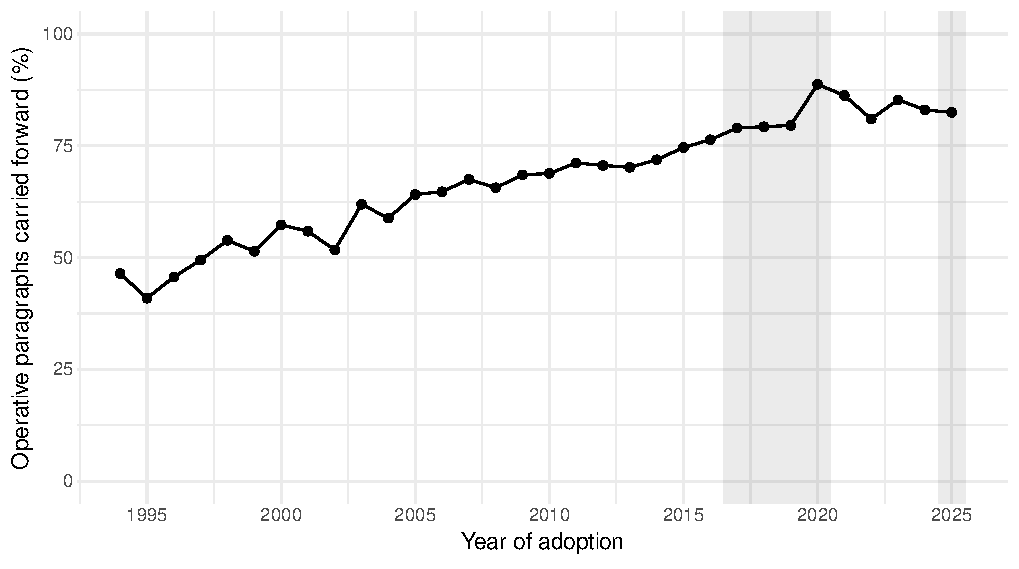
\includegraphics[width=\textwidth]{text_carried_forward.pdf}
\caption{Share of a predecessor's operative paragraphs carried forward into the next resolution of the same title, by year of adoption, 1994--2025. Each point averages the pairs of resolutions adopted in that year, with each pair weighted equally. A paragraph is carried forward when at least 80 percent of its distinct four-word sequences recur in the successor. Shading marks the first Trump administration (2017--2020) and the first year of the second (2025).}
\label{fig:text-carried-forward}
\end{figure}
\FloatBarrier

The figure of 82.5\% is high when measured against the average historical figures for the re-adoption of previous operative paragraphs (see Figure~\ref{fig:text-carried-forward}). In 1995 on average only 40.9\% of the previous operative paragraphs of earlier resolutions were re-adopted, in 2005 this was 64.1\%, and in 2015 74.6\% was recorded. While in 2025 on average the vast majority of previous wording was re-adopted, only four years out of 32 scored higher than the 2025 average. \footnote{The four are 2020, 2021, 2023 and 2024. The supplement reports alternative matching rules and omission checks.}

Major revisions are recorded in the same way as before. Thus the 2025 human-rights resolution on Syria, adopted after the change of government in Syria, repeated none of its predecessor's operative paragraphs. However, unchanged words may carry a revised instruction, and deleting a request can reflect work already completed. Following the requested actions lets us distinguish these possibilities.

\subsection{Most of the previous requests for action continued}

Washington opposed every resolution the Second Committee produced in 2025. \footnote{The United States voted against all forty-one resolutions from the committee in 2025. It had voted no on seven in 2024 and six in 2023.} We read its adopted economic and development decisions from 2023 through 2025 to establish what members continued to authorize. The Group of 77 often sponsors these texts for developing-world members; their adoption concerns the Assembly's work, separately from the fourteen allies' votes. For each of the same 24 initiatives, we trace earlier requests into the subsequent decision and classify their outcomes in Table~\ref{tab:adopted-continuity}. \footnote{An initiative is a resolution or decision and its successors; 24 recur in all three years after internal programme decisions are excluded. The supplement gives the population and distinctions between year-to-year and within-year requests.}

The table gives each initiative equal weight, first calculating its share of earlier requests continuing unchanged and then averaging those shares. For 2024--2025 the average is 81.3 percent, against 76.5 percent for 2023--2024. In other words, most of the work requested in the earlier decisions continued unchanged in both years, including the year when American opposition expanded sharply. These are substantive classifications of the requested actions, their recipients and conditions; the vote and wording measures alone cannot supply them. \footnote{The supplement details manual request coding, matching, classification and source checks.}

\begin{table}[!ht]
\centering
\caption{Outcomes of requests in the earlier adopted decision, one and two years later}
\label{tab:adopted-continuity}
\begin{tabularx}{\textwidth}{>{\raggedright\arraybackslash}Xccc}
\toprule
 & 2023 to 2024 & 2024 to 2025 & 2023 to 2025 \\
\midrule
Continued without substantive change & 76.5 & 81.3 & 67.4 \\
Continued with stronger requirements & 3.5 & 1.4 & 3.9 \\
Continued with weaker requirements & 1.1 & 0.6 & 1.2 \\
Changed, not comparable in strength & 3.4 & 5.1 & 7.5 \\
Completed or expired & 4.2 & 4.1 & 7.9 \\
No corresponding request & 0.5 & 0.5 & 1.1 \\
Unresolved & 10.8 & 7.1 & 11.0 \\
\addlinespace
Initiatives & 24 & 24 & 24 \\
Requests in the starting-year decisions & 873 & 870 & 873 \\
\bottomrule
\end{tabularx}
\begin{minipage}{.97\textwidth}\footnotesize Entries are percentages calculated within each initiative and then averaged across the same 24 initiatives. Unresolved requests stay in the denominator; added requests do not offset earlier ones. The two-year column compares 2023 and 2025 decisions directly, and rounding can prevent columns summing to 100.\end{minipage}
\end{table}
\FloatBarrier

Omitting initiatives one at a time still leaves most requests continuing unchanged; the supplement reports the ranges and the relationship to wording retention. Of course, the annual comparisons reuse texts and years, so we cannot treat their difference as a comparison of independent observations.

Some earlier work was completed or expired, an average of 4.1 percent of requests from 2024 to 2025. Other requests continued with stronger, weaker or different requirements, and 0.5 percent had no corresponding request. We retain the unresolved 7.1 percent in the denominator. Looking directly from 2023 to 2025 in the final column, 67.4 percent of earlier requests continued unchanged on average. \footnote{The supplement gives examples of each outcome, results for resource and reporting requests, comparisons omitting each initiative in turn, and the agreement between the request coding and the wording measure.}

Tax cooperation illustrates an earlier mandate continuing while votes change. Its resolution received 119 votes in favor and 9 against, with 43 abstentions, in 2024; in 2025 it received 122 in favor and 3 against, with 55 abstentions. Five allies moved from no to abstain, leaving all fourteen abstaining in 2025. Argentina and Israel voted no with the United States. The American delegation left the negotiating committee in February 2025. According to Eurodad, no other delegation followed it out of the session \citep{eurodad:2025:walkout}. The official report records later meetings and procedural decisions adopted without a vote \citep{un:2025:taxcommitteereport}. The shorter 2025 resolution retained the mandate, along with requests for Secretariat resources and developing-country participation. \footnote{Of 16 earlier requests, three are coded completed, three unchanged and ten unresolved. The mandate runs to 2027; the resolution's adoption is distinct from a completed convention.}

Development financing offers another case. After the United States withdrew from the Sevilla preparatory process, the conference adopted its outcome. All fourteen allies stayed in negotiations and voted in August 2025 to endorse the Sevilla Commitment in the Assembly, where it passed by 158 to 2 with one abstention. The United States and Israel voted no \citep{usun:2025:ffd4withdrawal,un:2025:sevillavote}. \footnote{The supplement gives the American withdrawal statement, the conference record and the Assembly's recorded vote.}

The coastal-ecosystems resolution of 2023 included a request to the developed countries to at least double adaptation finance by 2025 compared to the level of 2019 financing for adaptation. The earliest draft in 2025 still referred to this target. In the end however the adopted text of the request for action did not specify any actor, any amount of finance or any deadline. Thus there was no corresponding request for action for that earlier action. Most of the requested action, however, continued to be included in the adopted texts. \footnote{A/RES/78/159, para.~12, repeats the target in decision 1/CMA.3, para.~18, of the Glasgow climate conference. The omission records a change in the Assembly's text; establishing whether the underlying commitment ended requires further evidence.}

\subsection{Negotiation continued, including revisions sought by Washington}

For each of the years we trace all proposals from first consideration in text to adoption. Negotiations can be extensive while retaining much of an earlier agenda. All 128 of the substantive proposals and internal program decisions formally considered in main sessions of Second Committee in 2023-2025 years were in the end adopted, after considerable revision in each year. \footnote{The inventory covers formal consideration between September and December and excludes ideas abandoned before that stage. The supplement distinguishes Assembly resolutions, substantive decisions and internal committee decisions.} The average percentage of requests that survived in the adopted text as compared to the first issued draft was 81.7--87.7\% in 2025. For 2024 this average was 90.6--93.5\% and in 2023 on average 83.7--83.9\% of the requests contained in the first issued text had survived. Thus the degree of change as compared to previous years was higher in 2025 than in 2024 but similar to 2023. \footnote{The ranges reflect unresolved request classifications. For 26 proposals across the three years, nine in 2025, the first documented considered text was already a revision; the supplement reports both starting points.}

The United States participated actively. Its statement covered every Second Committee resolution. In that statement it sought to replace the general reaffirmation of the Sustainable Development Goals (SDGs) with specific development objectives. It also urged new initiatives to make use of existing resources. It also requested changes with respect to language on environment, sex and diversity issues. It opposed a UN role in international debt architecture and centralized UN mandates on artificial intelligence. \citep{usun:2025:longform}

In the vulnerability-index negotiation, a replacement draft issued six days after the American statement made two proposed appointments subject to existing resources, as Washington had recommended. It kept the time frames and a separate request for adequate resources. Nevertheless, the US voted against this decision. \footnote{Timing establishes that the revision followed the American demand, without identifying who secured it. The supplement and archive record the illustrative cases and their selection.}

Decisions in 2025 combined continuity, negotiated revisions and some lost requests. The Assembly retained most earlier requested work over American opposition. Some revisions matched American recommendations, as the example of the vulnerability-index negotiation demonstrates.

\section{Discussion}

The allies' response to the American reversal was to continue working together in the General Assembly. They largely kept their votes on recurring questions, maintained agreement with one another, and supported economic and development decisions over American opposition. Reading those decisions matters for the interpretation: most earlier requests for work continued, even where negotiation produced revisions. A fall in American agreement thus accompanied cooperation among its partners and other members who could still authorize work together.

Theories of cooperation after hegemony give us good reasons to expect institutions to outlast a decline in the original sponsor's power \citep{keohane:1984,snidal:1985}. The American reversal brings a further distinction into view, between its current policy leadership and support for activities within its order. Governments continued the tax negotiations and endorsed Sevilla after Washington withdrew its support. We can see their willingness to pursue the work in the decisions themselves. Of course, their first-year votes could also reflect patient bargaining with an American government whose policies they expected to change again. The origins of policy support and its expected duration require evidence beyond this first response.

The observed trade figures are also informative about relationships among the allies during this period. Their share of American merchandise imports fell from 36.3 percent in 2024 to 34.0 percent in 2025. Yet close to 51 percent of their non-US exports went to other allies in both years, with intra-allied exports rising 6.21 percent in nominal dollars. Eight members' shares fell, so the aggregate should not be read as a common experience across countries. The flows document continued exchange among allies as their share of the American market declined. They span the tariff changes described in the supplement \citep{crs:2025:tariffs,canada:2025:countertariffs}; estimating their effects would require a different design.

The Assembly gives governments a way to act on Carney's appeal to middle powers. They can use majority rule to authorize work and familiar procedures to renew mandates and negotiate revisions, as they did in 2025 over American opposition. The more difficult decisions may come when that work requires resources Washington supplies or action it can block. This is where authorization must be followed by financing and implementation. The first year establishes that members could keep deciding together after the hegemon reversed its policies; later years will show what they do as the costs of disagreement accumulate.

\setlength{\parskip}{0pt}
\newpage
\singlespacing
\small
\bibliographystyle{elsarticle-harv}
\bibliography{references}
\end{document}
